\section{Injury Conditions}\label{injuries}

\noindent To analyse the severity of the outcome from someone falling or bouncing off a trampoline at different heights, the forces at which bones in the body break must be calculated. Different injuries may be categorised to state their severity. For the purpose of this report, a fracture, break in a bone or concussion is considered to be serious, and a bruise is considered a minor injury. Being able to distinguish between these categories and see the forces which result in each provides some threshold that dictates the boundaries between no injury, minor, and serious injury.%% rewording
\\
\\
\noindent To compare vaulting injuries to those from trampolining is justifiable. Both sports expect falls from heights found to cause various levels of injuries, found to be average at 1.4m in the case of vaulting \cite{gcalc}. From the Results discovered in Section \ref{results}, the heights observed can be far greater in trampolining, this seems to be a good reference point to observe the forces that cause concern from this height and an intuitive assumption can be made that a fall from a greater height will be somewhat more damaging. Risk management guidelines for vaulting \cite{gcalc} suggest the forces that should not be exceeded for the following:

\begin{itemize}
\item 45g for children.
\item 65g for mature women.
\item 75g for mature men.
\item A force of 200g is unacceptable in any situation.
\end{itemize}

\noindent A few considerations are required when using this comparison regarding the people involved in each sport. For the purpose of this report the trampolines are being considered to be household trampolines, and those using them to be children and adults who are not likely to be professionals. The vaulters discussed are trained and know how to perform a 'bail-out' roll, in which the vaulter performs a forward roll out of the jump in order to reduce the risk of injury to the head. This is something that relies on, and also increases, the performers reflexes. This means that although the comparison between vaulter and trampolinist injuries are suitable, it would be expected that the trampolinist does not have sharp reflexes. If falling were to occur, they could be more prone to head injuries than a vaulter.
\\
\\
\noindent It is also important to note that, when falling off a trampoline, a person is exposed these g forces stated for a very short period of time. Prolonged exposure to g-forces lower than those stated above can result in serious injury, such as burst blood vessels and loss of consciousness \cite{gs}, the thresholds for injuries for a child are noted, and a serious injury will occur from 45g upwards from a fall, a lesser form of injury will occur below this value.
\\
\\
%\noindent To give an idea of the forces at which bones in the human body break, Medscape had produced an article on the g forces at which facial bones fracture.\cite{faceinjure}. The most significant data shown states that it would take around 30g of force to fracture the nasal bone, and 100g of force to cause a midline fracture the mandible. Another source had produced results that show that the pelvis fractures between 100 and 200g, and the vertebra compress and give fractures around 20 to 30g\cite{theback}. Children's bones are generally weaker as they are still growing and not fully developed and therefore more prone to breaking. This can be represented by a decrease of 38\% in the yield stress a child's bone can be subject to \cite{bonecomp}.% force = stress*area so do we need to calculate the area decrease in bone as well? can find an average for say a 5 year old or 10 year old and use these to find the forces.
\noindent To find the g force, $g_f$ acting on the body when coming into contact with the ground from falling from a height \cite{gcalc}, Equation (\ref{gforce}) is used:

\begin{equation}\label{gforce}
g_f=\frac{h}{d_s}
\end{equation}



\noindent Where $h$ is the height from which the person falls from. When considering the model this will be from the highest point the mass reaches in its trajectory. It is important to remember to add the height of the trampoline to this distance. The stopping distance, $d_s$ is the distance the ground surface adds to decelerate the mass falling into it to zero velocity.

\subsection{Injury Threshold Graph}

\noindent Knowledge of the stopping distance for a surface means that this injury threshold graph can be plotted based on what height the mass falls from. This is discussed in Section \ref{futureinjury}. Figure \ref{fig:inj} below shows the injury categories for falling from a height of 3 metres, including 1 metre from the height of the trampoline itself. Choosing the serious injury threshold to be 45g, as in Section \ref{futureinjury}, gives a stopping distance of 0.667 metres, using Equation (24), for an unspecified surface. This provides a clear visual representation of when serious injuries will occur for the given surface, a useful tool for a parent deciding where to place their trampoline and also allows them to see when their children are bouncing too high.

\begin{figure}[H]
	\centering
	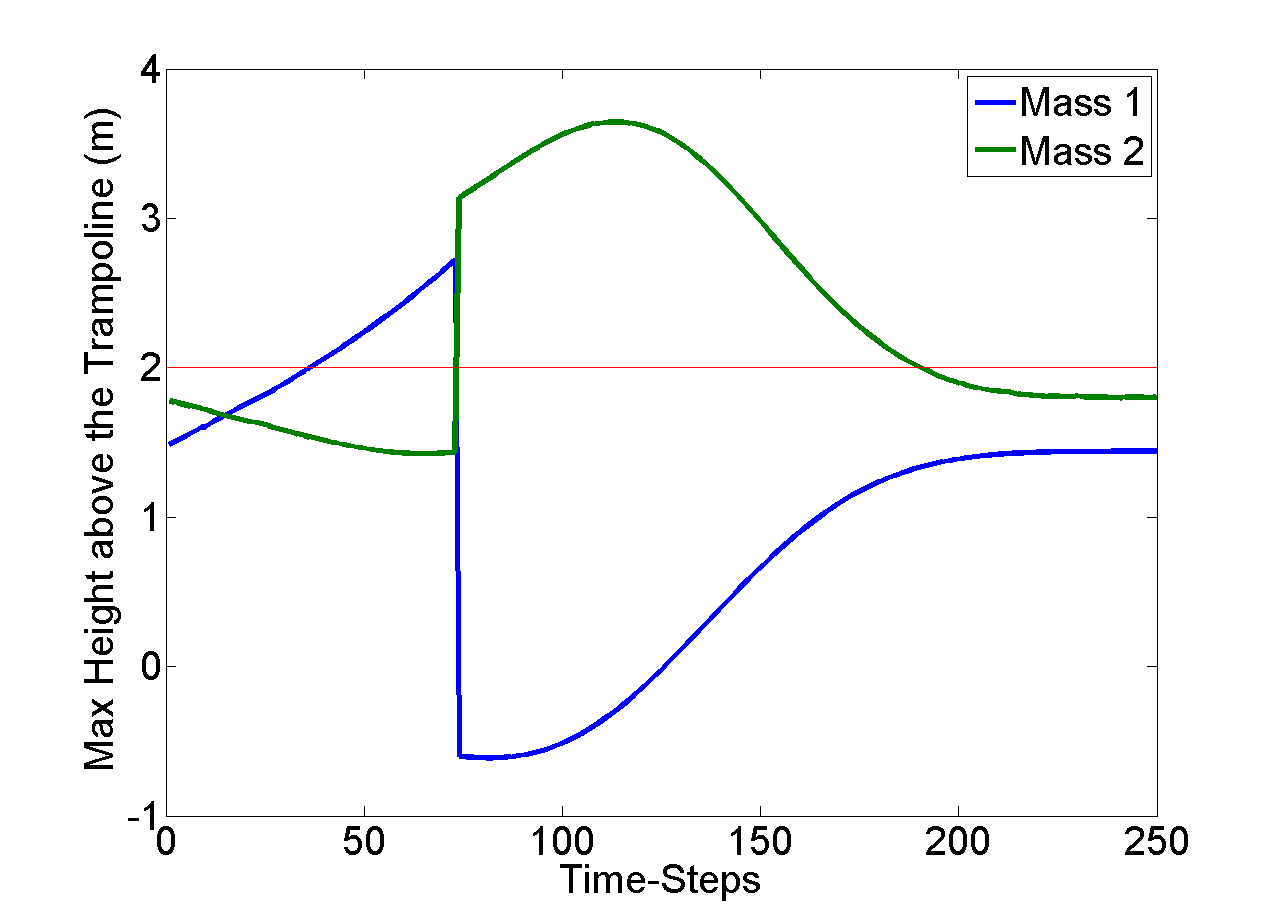
\includegraphics[width=3.1in, height=2in]{injury.png}
    \caption{A graph showing the serious injury threshold, represented by the red line, on the maximum heights reached by $m_1$ and $m_2$ when $m_1$ starts on the trampoline.}\label{fig:inj}
\end{figure}




% The amount of pressure required to break the femur, the strongest bone in the body, is over 1'000'000$kgm^{-2}$\cite{fibia}. However the amount of pressure to fracture the weakest bone in the body, the stapes, an ear bone is only 100'000$kgm^{-2}$. To cause brain damage and brain injury, one needs to exceed 50g in force.\cite{carcrash}



%to calculate the g forces on a body one has to combine the following equations; $v=\sqrt{2g_ch}$, $a=\frac{v^2}{2d_s}$ and $g_F=\frac{a}{g_c}$ where $v$ is the velocity at impact, $g_c$ is the acceleration due to gravity, $h$ is the height at which the object falls, $a$ is the deceleration produced, $d_s$ is the stopping distance, and $g_F$ is the g force.\cite{gcalc}
